\documentclass[a4paper, notitlepage, 10pt]{article}
\usepackage{geometry}
% WSC 2015 configs
\fontfamily{times}
\geometry{verbose,tmargin=30mm,bmargin=25mm,lmargin=25mm,rmargin=25mm}
% end configs
\usepackage{setspace,relsize}               
\usepackage{moreverb}                        
\usepackage{url}
\usepackage{hyperref}
\hypersetup{colorlinks=true,citecolor=blue}
\usepackage{amsmath}
\usepackage{mathtools} 
\usepackage{amsthm}
\usepackage{amssymb}
\usepackage{indentfirst}
\usepackage{todonotes}
\usepackage[authoryear,round]{natbib}
\bibliographystyle{apalike}
\usepackage[pdftex]{lscape}
\usepackage[utf8]{inputenc}

% Title Page
\title{\vspace{-9ex}\centering \bf Transform then pool or pool and then transform?}
\author{
Luiz Max F. de Carvalho\\
% Program for Scientific Computing (PROCC), Oswaldo Cruz Foundation. \\
% Institute of Evolutionary Biology, University of Edinburgh.\\
}
\DeclareMathOperator*{\argmin}{arg\,min}
\DeclareMathOperator*{\argmax}{arg\,max}
\newtheorem{theo}{Theorem}[]
\newtheorem{proposition}{Proposition}[]
\newtheorem{remark}{Remark}[]
\newtheorem{corollary}{Corollary}[]
\newtheorem{definition}{Definition}[]
\setcounter{theo}{0} % assign desired value to theorem counter
\begin{document}
\maketitle

\begin{abstract}
In this note I discuss the order of operations between transforming and pooling a set of distributions in relation to whether the transform in question is invertible.
I give an explicit example where both procedures lead to the same density even when the transform is not invertible and also discuss an example where the transform-then-pool and pool-then-transform with a non-invertible transform lead to distributions in the same family which are nonetheless distinct.
The lesson to be learned is that while the order of operations usually matters, it may not, depending on the distributions under consideration.

Key-words: logarithmic pooling; transformations; log-normal. 
\end{abstract}

\section*{TODO}
\begin{itemize}
 \item Get rid of all abuse of notation. 
 The statement $ \phi(\mathcal{LP}(\mathbf{F_X}, \boldsymbol\alpha)) = \pi_{Y}(y | \boldsymbol\alpha)$ is an abomination.
 \item Clearly establish the conditions under which $\phi()$ produces a pushforward measure that admits Radon-Nikodym derivatives. 
 Without this, it becomes meaningless to talk about ``induce-then-pool''; you can only pool proper probability densities and thus one needs to guarantee said densities in fact exist.
 \item Maybe formulate a measure-theoretic version of LP to deal with the difficulties above.
\end{itemize}


\section*{Background}

Logarithmic pooling is a popular method for combining opinions on an agreed quantity, specially when these opinions can be framed as probability distributions.
Let $\mathbf{F_\theta} := \{f_0(\theta), f_1(\theta), \ldots, f_K(\theta)\}$ be a set of distributions representing the opinions of $K + 1$ experts and let $\boldsymbol\alpha :=\{\alpha_0, \alpha_1, \ldots, \alpha_K \} \in \mathcal{S}^K$ be the vector of weights, such that $\alpha_i > 0\: \forall i$ and $\sum_{i=0}^K \alpha_i = 1$, i.e., $\mathcal{S}^{K + 1}$ is the space of all open simplices of dimension $K + 1$.
The \textbf{logarithmic pooling operator} $\mathcal{LP}(\mathbf{F_\theta}, \boldsymbol\alpha)$ is defined as
\begin{equation}
\label{eq:logpool}
 \mathcal{LP}(\mathbf{F_\theta}, \boldsymbol\alpha) :=  \pi(\theta | \boldsymbol\alpha) = t(\boldsymbol\alpha) \prod_{i=0}^K f_i(\theta)^{\alpha_i},
\end{equation}
where $t(\boldsymbol\alpha) = \left[ \int_{\boldsymbol\Theta}\prod_{i=0}^K f_i(\theta)^{\alpha_i}d\theta \right]^{-1}$.
This pooling method enjoys several desirable properties and yields tractable distributions for a large class of distribution families~\citep{genest1984,genest1986A,Carvalho2019}.

\section*{Pool then transform or transform and then pool?}

Suppose the we are interested in the distribution of a random variable $Y \in \mathcal{Y}\subseteq \mathbb{R}^q$  when one has a random variable $X \in \mathcal{X} \subseteq \mathbb{R}^p$ with $\phi : \mathcal{X} \to \mathcal{Y}$.
Let $|J_\phi|$ be the (absolute) Jacobian determinant w.r.t. $\phi$.
Suppose further that each expert $i$ produces a distribution $f_i(X)$ such that we can construct the object $\mathbf{F}_X = \{f_1(X), f_2(X), \ldots, f_K(X) \}$.
Then one can either:
\begin{itemize}
 \item[(a)] \textbf{Pool-then-transform:} construct $\pi_X(X | \boldsymbol \alpha) = \mathcal{LP}(\mathbf{F}_X, \boldsymbol \alpha)$ and then apply $\phi$ to obtain $\pi_Y(Y | \boldsymbol \alpha) := \pi_X( \phi^{-1}(Y)| \boldsymbol\alpha) |J_\phi|$;
 \item[(b)] \textbf{Transform-then-pool:} apply the transform to each component $i$ of $\mathbf{F}_X$ to build
 \[\mathbf{G}_{Y}:= \{g_i(Y), g_2(Y), \ldots, g_K(Y)\} \]
 and obtain $\pi_Y^{\prime}(Y |  \boldsymbol \alpha) = \mathcal{LP}(\mathbf{G}_{Y},  \boldsymbol \alpha)$.
\end{itemize}

First, let us start with a couple definitions
\begin{definition}
Let $A, B \subseteq \mathbb{R}^p$.
A function  $h: A \to B$ is \textbf{invertible} iff $\: \exists \: h^{-1}: B \to A \: \text{with} \: h^{-1}(h(a)) = a \: \forall \: a \in A$. 
Let $\pi_A$ be an arbitrary probability measure in A. 
If $h$ is monotonic and differentiable we can write $\pi_B(B) = \pi_A(h^{-1}(A))|J|$, where $|J|$ is the absolute determinant of the Jacobian matrix with entries $J_{ik} := \partial h_k^{-1}/\partial a_i$, $i,k = 1, 2, \ldots, p$.
\end{definition}

\begin{definition}
 Let $f$ and $g$ be probability density functions with support on $\mathcal{X} \subseteq \mathbb{R}^d$.
 We say $f \equiv g$ if $f(x) = g(x)$ for almost every point $x \in \mathcal{X}$, that is, \textit{almost everywhere, a.e.}
 This is equivalent to stating that $\mu(A) = 0$ where $A := \{ x \in \mathcal{X} : f(x) \neq g(x) \}$ and $\mu$ is the dominating measure.
\end{definition}
\begin{remark}
\label{rmk:invariance}
If $\phi$ is invertible, then $\pi_Y \equiv \pi_Y^{\prime}$.
\end{remark}
\begin{proof}
First, 
\begin{align}
 \pi_Y(y | \boldsymbol \alpha) & \propto \pi_{X}(\phi^{-1}(y))|J_\phi|, \\
&= \prod_{i = 0}^K \left[ f_i(\phi^{-1}(y)) \right]^{\alpha_i}|J_\phi|.
\end{align}
For situation (b) we have:
\begin{equation}
 g_i(y) = f_i(\phi^{-1}(y))|J_\phi|.
\end{equation}
And,
\begin{align}
 \pi_Y^{\prime}(y |  \boldsymbol \alpha) & \propto  \prod_{i=0}^K g_i(y)^{\alpha_i} \\
  & =  \prod_{i=0}^K \left[ f_i(\phi_x^{-1}(y))|J_\phi| \right]^{\alpha_i} \\
  & = \prod_{i = 0}^K \left[ f_i(\phi^{-1}(y)) \right]^{\alpha_i}|J_\phi|,
\end{align}
as claimed.
\end{proof}
\begin{corollary}
\label{clr:inverseGamma}
 The log-pooled distribution from a collection of inverse-Gamma densities with parameters $\eta_i$, $\beta_i$ is inverse-Gamma with parameters $\eta^\star = \sum_{i = 0}^K \alpha_i \eta_i$ and $\beta^\star = \sum_{i = 0}^K \alpha_i \beta_i$.
\end{corollary}
\begin{proof}
First, recall that if $X \sim \text{Gamma}(a, b)$ then $ 1/X \sim \text{Inverse-Gamma}(a, b)$.
\cite{Carvalho2019} show that if the $f_i$ are Gamma densities  with parameters $\eta_i$ and $\beta_i$ (shape/rate parametrisation) then the pooled distribution is a Gamma distribution with parameters $\eta^\star = \sum_{i = 0}^K \alpha_i \eta_i$ and $\beta^\star = \sum_{i = 0}^K \alpha_i \beta_i$.
Since $\phi(x) = 1/x$ is invertible, the result follows from Remark~\ref{rmk:invariance}.
\end{proof}
While Corollary~\ref{clr:inverseGamma} is straightforward to get by direct calculation, our goal here is to illustrate how Remark~\ref{rmk:invariance} could be used in situations where direct calculation is unwieldly.
An interesting idea is whether Remark~\ref{rmk:invariance} is an ``if and only if'' (iff) result.
As we shall see, the answer is no (Remark~\ref{rmk:invertibleIFF}).
% Let $\phi : \mathcal{X} \to \mathcal{Y}$ be a surjective non-injective differentiable function, which is not invertible on the whole of $\mathcal{Y}$, but instead is \textbf{piece-wise invertible}.
% Let $\mathcal{Y}_1, \mathcal{Y}_2, \ldots, \mathcal{Y}_T$ be a  partition of $\mathcal{Y}$, i.e., $\mathcal{Y}_i\cap\mathcal{Y}_j = \emptyset,\: \forall i\neq j \in \{1, 2, \ldots, T\}$ and $\bigcup_{t = 1}^T\mathcal{Y}_t = \mathcal{Y}$.
% Then define the inverse functions $\phi_{t}^{-1}(y)\,:\, \mathcal{Y}_t \to \mathcal{X}, \: t \in \{1, 2, \ldots, T\}$.
% Lastly, let $|J_t|$ be the Jacobian of $\phi_{t}^{-1}(\cdot)$.
% Then we are prepared to write:
% \begin{align}
% \label{eq:piecewiseTransf}
% \pi_{Y}(y |\boldsymbol\alpha) &\propto \sum_{t = 1}^T\left(\prod_{i=0}^K f_i(\phi_t^{-1}(y))^{\alpha_i}\right)|J_t| \quad \text{and}\\
% \pi^{\prime}_{Y}(y|\boldsymbol\alpha) &\propto \prod_{i=0}^K\left[\sum_{t = 1}^T f_i(\phi_t^{-1}(y))|J_t|\right]^{\alpha_i}
% \end{align}
% which, I claim, will only be equal if $T = 1$, i.e. if $\phi(\cdot)$ is invertible in the usual sense.
% Below I try to establish a result in general for any surjective non-injective mapping, not just piece-wise invertible ones.
\begin{remark}
 \label{rmk:invertibleIFF}
 It is possible to have  $\pi_Y \equiv \pi_Y^{\prime}$ even when $\phi$ is not invertible.
\end{remark}
\begin{proof}
We will show this by way of an explicit example.
In general, we can define 
\begin{equation}
 g_i(y) = \sum_{\omega \in \Omega(y)} \frac{f_i(\omega)}{|\phi^\prime(\omega)|}.
\end{equation}
where $\Omega(y) := \{ x: \phi(x) = y \}$ \footnote{Notice there is no guarantee that $|\Omega(y)| < \infty$.}.
Notice that for any $x \in \mathcal{X}$, there exists $y$ such that $x \in \Omega(y)$. 
Assume that the transform $\phi$ is non-invertible, i.e., that $|\Omega(y)| > 1$ for some $y \in \mathcal{Y}$, and $f_i \not\equiv f_j,$ for some $i, j$.
We have
\begin{align}
\label{eq:generalTransf}
\pi_{Y}(y |\boldsymbol\alpha) &= T(\boldsymbol\alpha) \sum_{\omega \in \Omega(y)} \frac{\prod_{i=0}^K f_i(\omega)^{\alpha_i}}{|\phi^\prime(\omega)|}
\quad \text{and}\\
\pi^{\prime}_{Y}(y|\boldsymbol\alpha) &= T^\prime(\boldsymbol\alpha)  \prod_{i=0}^K g_i(y)^{\alpha_i} = T^\prime(\boldsymbol\alpha)  \prod_{i=0}^K\left[\sum_{\omega \in \Omega(y)} \frac{f_i(\omega)}{|\phi^\prime(\omega)|}\right]^{\alpha_i},
\end{align}
with
\begin{equation*}
 T(\boldsymbol\alpha)  = \int_{\mathcal{Y}} \sum_{\omega \in \Omega(y)}\prod_{i=0}^K \left(\frac{f_i(\omega)}{|\phi^\prime(\omega)|}\right)^{\alpha_i}dy = \int_{\mathcal{X}}  \prod_{i=0}^K f_i(x)^{\alpha_i} dx \quad \text{and} \quad T(\boldsymbol\alpha)^{\prime}= \int_{\mathcal{Y}} \prod_{i=0}^K\left[\sum_{\omega \in \Omega(y)} \frac{f_i(\omega)}{|\phi^\prime(\omega)|}\right]^{\alpha_i} dy.
\end{equation*}
Now let us construct an explicit example.
Let $X$ be a quantity of interest and let $\boldsymbol F_X$ be such that each $f_i$ is a Gaussian density with zero mean\footnote{This is important so we can employ a symmetry argument later on.} and variance $v_i$, i.e.,
\[ f_i (x) = \frac{1}{\sqrt{2\pi v_i}} \exp\left(-\frac{x^2}{2v_i}\right) \]
Now consider $\phi(x) = x^2$ and  $Y = \phi(X)$.
Clearly, $\Omega(y) = \{ \omega_0, \omega_1 \} = \{ -\sqrt{y}, \sqrt{y} \}$ and hence
\begin{align}
 \label{eq:normalInvert}
 g_i(y) &= \frac{f_i(\omega_0)}{|2\omega_0|} + \frac{f_i(\omega_1)}{|2\omega_1|}, \\
        &= \frac{f_i(\sqrt{y})}{\sqrt{y}} = \frac{1}{\sqrt{2\pi v_i y}} \exp\left(-\frac{y}{2v_i}\right).
\end{align}
where the second line follows by using the symmetry of the Gaussian density around zero.
We are now prepared to write 
\begin{equation}
 \pi_Y(y |  \boldsymbol \alpha) = \frac{1}{\sqrt{2\pi v^\ast y}} \exp\left(-\frac{y}{2v^\ast}\right). \\
\end{equation}
whence $v^\ast =  \left[\sum_{i=0}^K \frac{\alpha_i}{v_i} \right]^{-1}$.
This follows from the pool of log-normals being also a log-normal -- see the Appendix of~\cite{Carvalho2019} for the derivation.
An explicit computation gives $\pi^{\prime}_{Y}$:
\begin{align}
 \pi^{\prime}_{Y}(y|  \boldsymbol \alpha) &\propto \prod_{i=0}^K g_i(y)^{\alpha_i}, \\
 & \propto \prod_{i=0}^K \left( \frac{1}{\sqrt{2\pi v_i y}} \right)^{\alpha_i} \exp\left(-\frac{\alpha_i y}{2v_i}\right),\\
 &= \frac{1}{\sqrt{2\pi v^\ast y}} \exp\left(-\frac{y}{2v^\ast}\right).
\end{align}
which establishes $ \pi_{Y}(y|  \boldsymbol \alpha) =  \pi^{\prime}_{Y}(y|  \boldsymbol \alpha)$ for any $ y \in \mathcal{Y}$.
\end{proof}
% There probably exists a measure-theoretic proof that is way more elegant, but this should suffice.
See Figure~\ref{fig:normal_square_example} for graphical depiction of the example given above.
We could have chosen any distribution on $(-\infty, \infty)$ symmetric about $0$.
This result shows that it is indeed possible to obtain the same density even when $\phi$ is not one-to-one.

\begin{figure}[!ht]
\centering
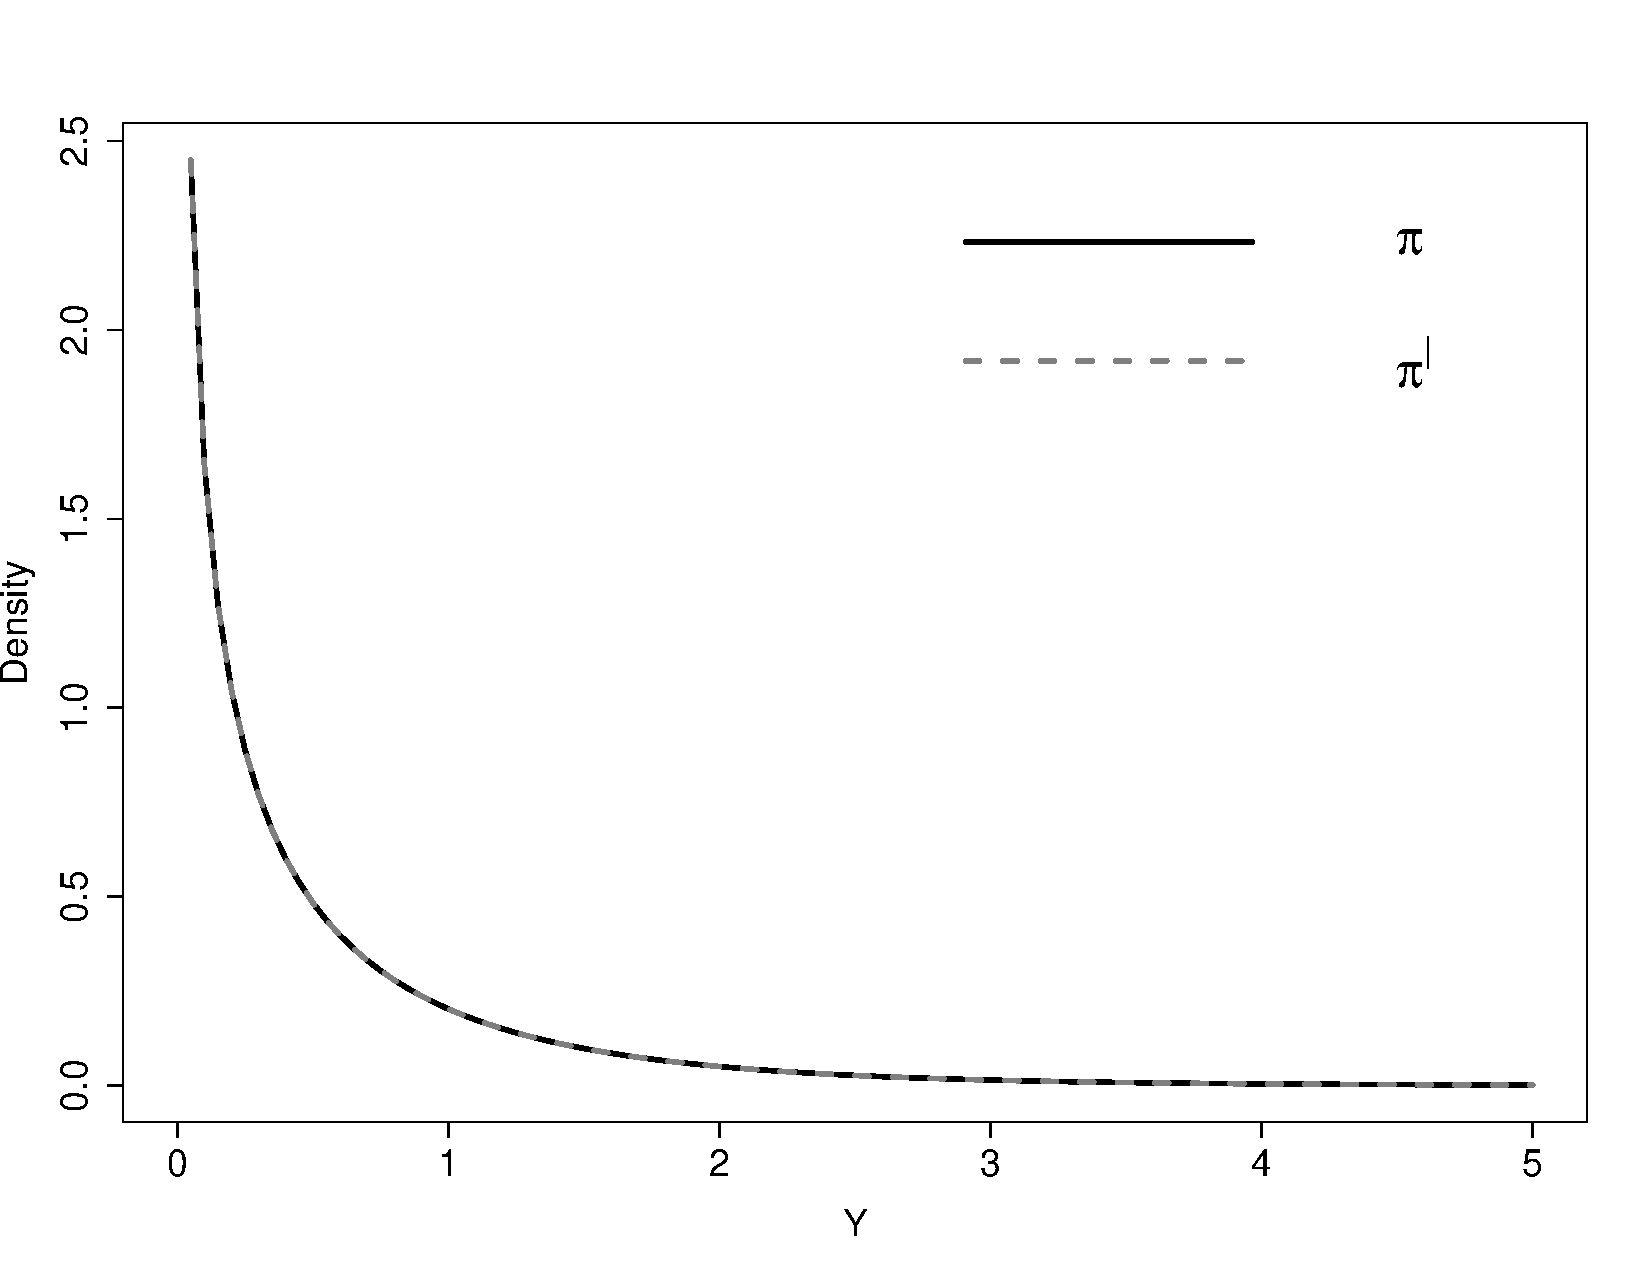
\includegraphics[scale=0.5]{figures/normal_square_example.pdf}
\caption{\textbf{Equivalent densities under a non-invertible transform}. Solid line displays $\pi_Y(Y | \boldsymbol\alpha)$, obtained by first pooling the distributions on $X$ and then computing the induced distribution on $Y$.
Dashed line displays the logarithmic pooling of individual distributions $g_{i}$, $\pi_Y^{\prime}(Y | \boldsymbol\alpha)$.
For this example $K=5$, $\boldsymbol \alpha = \{0.31, 0.08, 0.39, 0.08, 0.15 \} $, $\boldsymbol v = \{ 0.25, 0.75, 1.00, 1.00, 0.50 \}$.
}
\label{fig:normal_square_example}
\end{figure}

\newpage
\section*{An example where the two approaches are \textbf{NOT} the same}

The order of operations, i.e., whether one adopts procedure (a) or procedure (b), will likely affect the resulting densities, however.
In this section we will discuss an example where both procedures lead to densities in the same family, namely the log-normal family of distributions, which are nonetheless distinct.

Suppose $Z = U/V$ and each expert $i$ elicits $U \sim \text{log-normal}(\mu_{iU}, \sigma_{iU}^2)$, $V \sim \text{log-normal}(\mu_{iV}, \sigma_{iV}^2)$, i.e.
\begin{eqnarray*}
\nonumber
f_{iU}(u | \mu_{iU}, \sigma_{iU}^2) &=& \frac{1}{u \sqrt{2\pi\sigma_{iU}^2}} \exp\left( - \frac{ \left( \ln u - \mu_{iU} \right)^2 }{2 \sigma_{iU}^2} \right), \\
g_{iV}(v | \mu_{iV}, \sigma_{iV}^2) &=& \frac{1}{v \sqrt{2\pi\sigma_{iV}^2}} \exp\left( - \frac{ \left( \ln v - \mu_{iV} \right)^2 }{2 \sigma_{iV}^2} \right).
\end{eqnarray*}
Again, let $\mathbf{F}_U = \{f_{1U}(U), f_{2U}(U), \ldots, f_{KU}(U) \}$ and $\mathbf{G}_V = \{g_{1V}(V), g_{2V}(V), \ldots, g_{KV}(V) \}$.
First, let us derive $\pi_Z(Z)$ under scheme (a).
It is not hard to show that  $\pi_U(U | \boldsymbol\alpha) := \mathcal{LP}(\mathbf{F}_{U}, \boldsymbol \alpha) =  \text{log-normal}(\mu_U^\ast, v_U^\ast)$ with
\begin{align}
 \mu_U^\ast &:= \frac{\sum_{i=0}^K w_{iU} \mu_{iU}}{\sum_{i=0}^K w_{iU}}, \\
 v_U^\ast &:= \frac{1}{\sum_{i=0}^K w_{iU} }, \\
 w_{iU} &:=  \frac{\alpha_i}{\sigma_{iU}^2}.
\end{align}
See~\cite{Carvalho2019} for a proof.
Analagously, $\pi_V(V | \boldsymbol\alpha) := \mathcal{LP}(\mathbf{G}_{V}, \boldsymbol \alpha) =  \text{log-normal}(\mu_V^\ast, v_V^\ast)$.
Then $\pi_Z(Z |  \boldsymbol \alpha) = \text{log-normal}(\mu_Z^{\ast}, v_Z^{\ast})$, with
\begin{align}
\nonumber
 \mu_Z^{\ast} &= \mu_U^\ast - \mu_V^\ast,\\
 &= \frac{\sum_{i=0}^K w_{iU} \mu_{iU}}{\sum_{i=0}^K w_{iU}} - \frac{\sum_{i=0}^K w_{iV} \mu_{iV}}{\sum_{i=0}^K w_{iV}}\quad \text{and} \\
 \nonumber
v_Z^{\ast} &= v_U^\ast + v_V^\ast, \\
&= \frac{1}{\sum_{i=0}^K w_{iU} } + \frac{1}{\sum_{i=0}^K w_{iV} }.
\end{align}
Now let us consider case (b).
Since $r_{iZ} = \text{log-normal}(\mu_{iU} - \mu_{iV}, \sigma_{iU}^2 +  \sigma_{iV}^2)$, we arrive at  $\pi_Z^{\prime}(Z |  \boldsymbol \alpha) = \text{log-normal}(\mu_Z^{\ast\ast}, v_Z^{\ast\ast})$,
\begin{align}
 \mu_Z^{\ast\ast} &:= \frac{\sum_{i=0}^K w_{iZ} \mu_{iU}}{\sum_{i=0}^K w_{iZ}} - \frac{\sum_{i=0}^K w_{iZ} \mu_{iV}}{\sum_{i=0}^K w_{iZ}}, \\
 v_Z^{\ast\ast} &:= \frac{1}{\sum_{i=0}^K w_{iZ} }, \\
 w_{iZ} &:=  \frac{\alpha_i}{\sigma_{iU}^2 + \sigma_{iV}^2}.
\end{align}
Clearly, $v_Z^{\ast} \leq v_Z^{\ast\ast}$ and hence $\mu_Z^{\ast\ast} \leq \mu_Z^{\ast} \: \forall \: \boldsymbol\alpha$. [NOPE. THIS AIN'T TRUE AT ALL. NEEDS REVISION].

\begin{figure}[!ht]
\centering
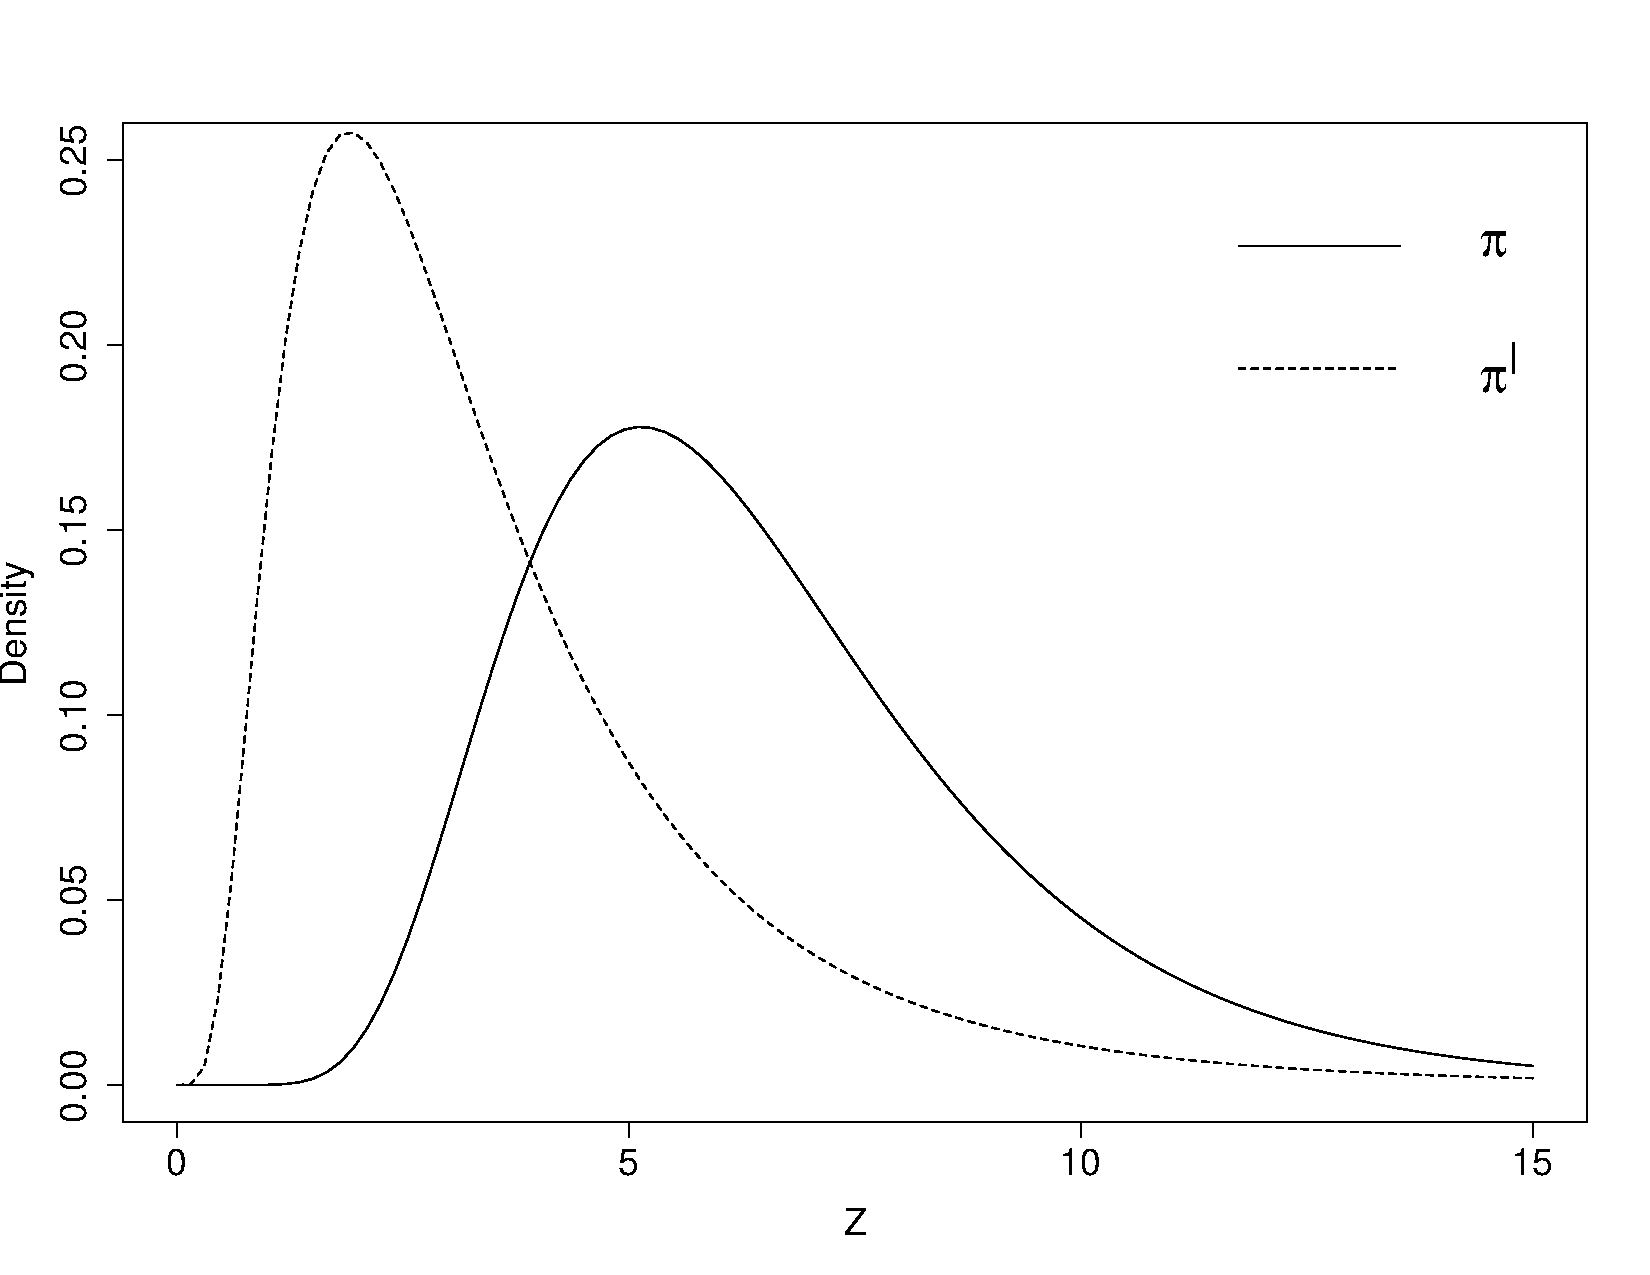
\includegraphics[scale=0.5]{figures/lognormal_example.pdf}
\caption{\textbf{Log-normal example}. Solid line displays $\pi_Z(Z | \boldsymbol\alpha)$, obtained by first pooling the distributions on $U$ and $V$ and then computing the induced distribution on $Z$.
Dashed line displays the logarithmic pooling of individual distributions $r_{iZ}$, $\pi_Z^{\prime}(Z | \boldsymbol\alpha)$.
For this example $K=2$, $\alpha_0 = 0.70$, $\mu_{0U} = 0.80$, $\sigma_{0U}^2 = 0.40$, $\mu_{1U} = 0.5$, $\sigma_{1U}^2 = 0.05$, $\mu_{0V} = -1.60$, $\sigma_{0V}^2 = 0.024$, $\mu_{1V} = -1.25$ and  $\sigma_{1V}^2 = 0.4$.
}
\label{fig:lognormal_example}
\end{figure}


\section*{Minimising Kullback-Leibler divergence in transformed space}

One might argue that procedure (b) makes little sense, given that the set of opinions $\mathbf{F}_{X}$ concerns only $X$, i.e, it was not necessarily constructed taking the transformation $\phi(\cdot)$ into account.
An example is a situation where experts are asked to provide distributions on the probability $p$ of a particular event.
In general, elicitation for $f_i(p)$ will not take into account the induced distribution on the log-odds, $\phi(p) = \log \left( p/(1-p) \right)$.
%% LM: we can change this dull example to something more involved.
% \[ f(l \mid a, b) = \frac{1}{\mathcal{B}(a, b)} \left(\frac{e^x}{e^x + 1}\right)^{a-1} \left(1- \frac{e^x}{e^x + 1}\right)^{b-1}\frac{e^x}{(e^x + 1)^2} \]
Nevertheless, the decision-maker may wish to assign the weights $\boldsymbol\alpha$ in a way that takes $\phi(\cdot)$ into account, e.g., by giving lower weights to experts whose distributions on the log-odds scale are unreasonable.

This decision process can be made more precise.
In a similar spirit to~\cite{Carvalho2019}, one can construct $\boldsymbol\alpha$ so as to minimise the Kullback-Leibler divergence between each distribution in $\mathbf{F^{-1}_y}$ and a transformation of the distribution obtained by procedure (a), $ \phi(\mathcal{LP}(\mathbf{F_X}, \boldsymbol\alpha)) = \pi_{Y}(y | \boldsymbol\alpha)$.
We aim at solving the problem
\begin{align}
L(\boldsymbol\alpha) &= \sum_{i=0}^K \text{KL}(  \pi_{Y} || h_i), \\
     \hat{\boldsymbol\alpha}:=& \:\argmin L(\boldsymbol\alpha)  \nonumber
\end{align}

This procedure therefore choses weights for each expert by how coherent the prior provided by each expert is with the pool-then-Transform -- procedure (a) -- prior in the transformed space induced by $\phi(\cdot)$.
When $\phi()$ is invertible, Remark~\ref{rmk:invariance} tells us that this procedure is the same as minimising the KL divergence between $\pi_X$ and each $f_i$, since the Kullback-Leibler divergence is invariant under invertible differentiable transformations.
Thus, in the probability/log-odds example mentioned above, the decision maker would not need to worry about the distributions on the log-odds induced by $\phi$, since it is invertible.


\section*{Acknowledgements}

LMFC is grateful to Mike West (Duke University) for not being impressed about the invertible case and prompting us to look at it in more detail.

\bibliography{../manuscript/pooling}

\end{document}          
